\documentclass{article}
\usepackage[T1]{fontenc}
\usepackage[utf8]{inputenc}
\usepackage[section]{placeins}
\usepackage{fullpage}
\usepackage{graphicx}
\usepackage{caption}
\usepackage{subcaption}

\graphicspath{ {./images/} }

\title{CS 4516 Group \#5: Bandwidth Trunking Using Layer 2 Devices\\Results}
\author{Jason Rosenman \and Louis Fogel \and Sam Abradi}
\date{}

\begin{document}
\maketitle
In order to measure the effectiveness of our approach, we will collect performance metrics on our switching approach.
We will compare the results of these metrics to the performance of an unmodified software switch.
Due to the fact that neither switch will be implemented in hardware, our results may be slightly different than a hardware implementation.
We are looking to compare the behavior of the network at saturation both with and without redundant links.
We are going to look at the goodput of these situations with and without congestion control.
\begin{figure}[ht]
	\centering
	\begin{subfigure}[b]{0.4\textwidth}
		\centering
		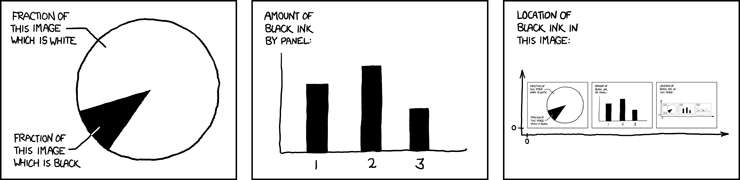
\includegraphics[scale=0.4]{self_description.png}
		\caption{Conventional Switch}
		\label{fig:stdbcast}
	\end{subfigure}
	\hfill
	\begin{subfigure}[b]{0.4\textwidth}
		\centering
		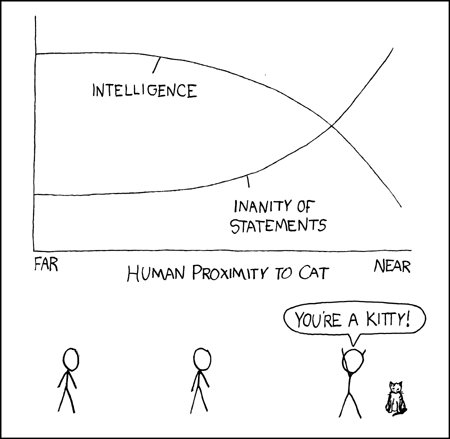
\includegraphics[scale=0.3]{cat_proximity.png}
		\caption{Smart Switch}
		\label{fig:newbcast}
	\end{subfigure}
	\caption{Percentage of Broadcast Traffic}
	\label{fig:bcast}
\end{figure}

Another useful metric is the percentage of broadcast traffic.
Normally (in a star network with conventional switches), nearly all of the traffic will start as broadcast traffic during the auto-configuration period.
The amount of broadcast traffic will then drop down to a noise-floor level.
If the network has a loop in it, the amount of broadcast traffic will not drop-off because the network will start a broadcast storm as a result of the forwarding loop.
We are looking for drop-off behavior in our switch, even in a graph network.


\section{Congestion Conditions}
We expect that situations where the network is at saturation will show the biggest difference in performance between architectures.
A setup with redundant links should perform much better than any other system if there is one flow causing all or most of the congestion, because all of the other traffic will default to the other link.
Clearly single links are unable to provide this service, so they are going to have horrible performance in congestion conditions.
\section{Congestion Control}
We have no idea what will happen in this situation.
The results will come from having hosts send traffic to eachother with an AIMD congestion controll model.
This may expose flaws in our bandwidth sharing, because links only hover near saturation, so the switch may have a hard time determining that more flows need to be moved over to the other link, because the flows will be too squishy.
\end{document}
